\chapter{Summary and Outlook}
In this thesis, we have measured the elliptic flow in 0--5\% centrality \pau collisions at \sqsn = 200 GeV. The elliptic flow is quantified by measuring the second-order flow coefficient $v_2$ defined as:
\begin{equation}
v_2 = \frac{\langle\cos 2(\phi-\Psi_2) \rangle}{ Res(\Psi_2)},
\end{equation}
where $\phi$ is the azimuthal angle of charged hadrons at mid-rapidity, $\Psi_2$ is the second-order event plane determined at backwards rapidity (Au-going direction), and Resolution$(\Psi_2)$ is the event plane resolution. This procedure is detailed in Section 4.2.1.

The measurement of $v_2(\pt)$, as a function of transverse momentum, in 0--5\% centrality \pau at \sqsn = 200 GeV collisions completes a set of measurements with engineered initial geometries at RHIC, including the \pau, \dau, and \hau as shown in Figure \ref{fig:all_system_hydro_6}. Sources of systematic uncertainty have been described in detail in Chapter 4, Section 4.5, with the non-flow being the dominant source of systematic uncertainty. The measured $v_2(\pt)$ in \pau at \sqsn = 200 GeV is in agreement with Monte Carlo Glauber initial conditions plus relativistic hydrodynamics (SONIC), as also shown in Figure \ref{fig:all_system_hydro_6}. The agreement of $v_2$ with a hydrodynamic model is an indication that the initial state geometry becomes transformed into a final state momentum anisotropy in 0--5\% \pau at \sqsn = 200 GeV collisions. 

\begin{figure}[!ht]
\begin{center}
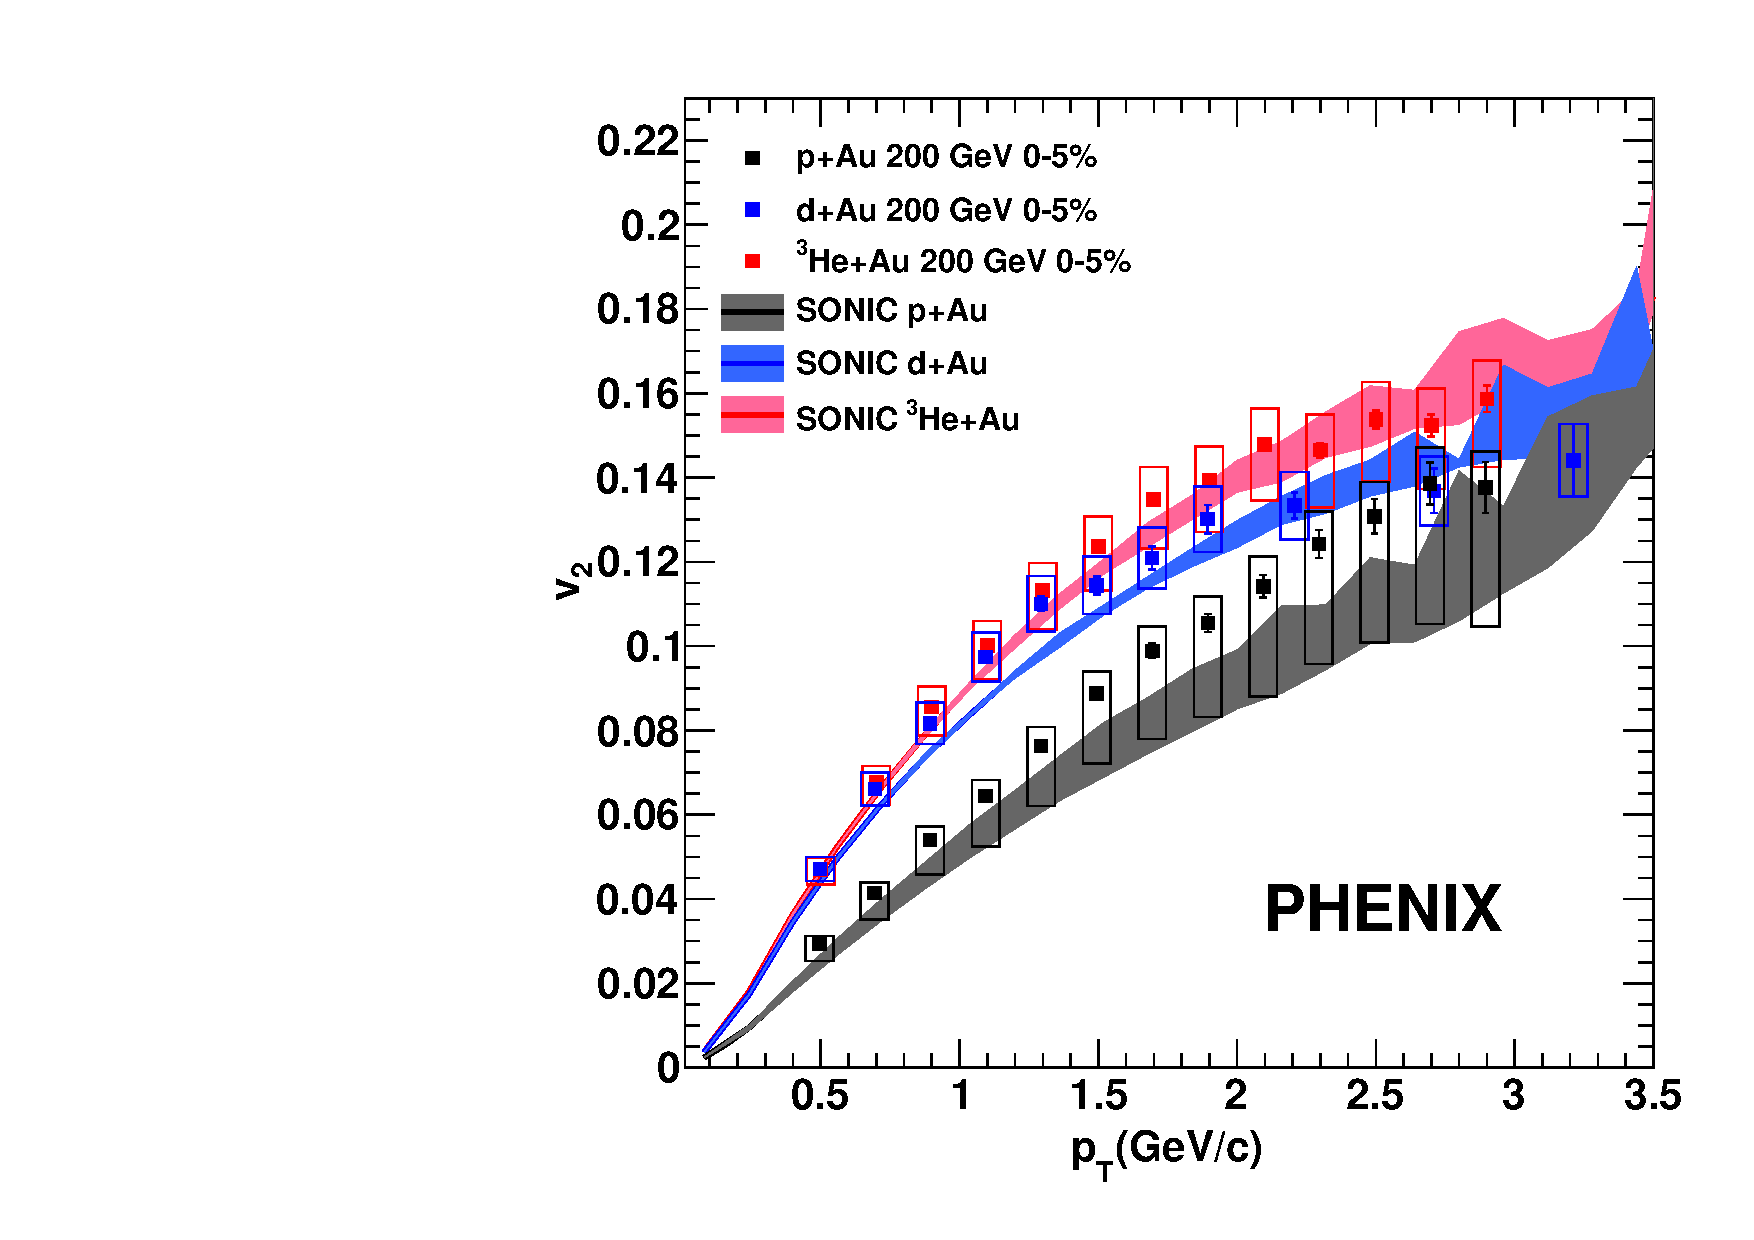
\includegraphics[width=0.5\linewidth]{figs/three_system_comparison_result.pdf}
\caption{$v_2$ of charged hadrons within $|\eta| <$ 0.35 in 0--5\% centrality \pau, \dau, and \hau at \sqsn = 200 GeV, compared with hydrodynamic calculations using the SONIC model, matched to the same multiplicity as the data~\cite{Habich:2014jna}.}
\label{fig:all_system_hydro_6}
\end{center}
\end{figure}

In order to properly compare the $v_2$ of \pau, \dau, and \hau at \sqsn = 200 GeV for each system, we have compared the average second-order eccentricity $\varepsilon_2$ of the initial collision, as defined in Section 5.3.1. If the measured $v_2$ is primarily from hydrodynamic flow, i.e. minimal levels of non-flow, then $v_2 \propto \varepsilon_2$. Thus, the MC-Glauber $\varepsilon_2$ for \pau, \dau, and \hau being 0.23, 0.54, and 0.50, respectively, implies the ordering of $v_2$ of the three systems should be $v_2^{\dau} \approx v_2^{\hau} > v_2^{\pau}$, which is what is observed in Figure \ref{fig:all_system_hydro_6}.
%\clearpage

Future work is being done in analyzing small collision systems recently run (in 2016) at RHIC: \dau at \sqsn = 200, 62.4, 39, and 19.6 GeV. By measuring the elliptic flow in this \dau beam energy scan, information on the effect of varying the initial temperature and the lifetime of the medium can be obtained. It is noteworthy that even at low \sqsn for \dau collisions, hydrodynamic simulations predict that the space-time volume of QGP is not negligible, as shown in Figure~\ref{fig:size_or_mediumcalc}~\cite{PhysRevC.93.044910}. In fact, the calculated space-time volume of the medium at \sqsn = 19.6 GeV is roughly half of the calculated space-time volume for \sqsn = 200 GeV, indicating that there is a reasonable expectation to see some evidence of a QGP medium forming in \dau collisions event at \sqsn = 19.6 GeV.

\begin{figure}[!ht]
\begin{center}
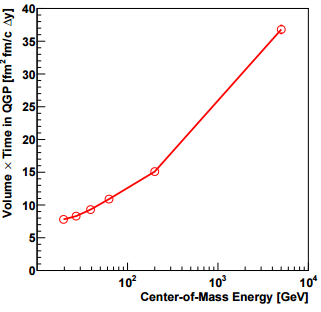
\includegraphics[width=0.5\linewidth]{figs/size_of_medium_calculation.png}
\caption{The total space-time volume as a function of \sqsn in heavy ion collisions calculated by a hydrodynamic model~\cite{PhysRevC.93.044910}.}
\label{fig:size_or_mediumcalc}
\end{center}
\end{figure}

Predications have been made of the $v_2$ for the various energies of the \dau beam energy scan by using the SONIC, superSONIC, and AMPT models; these models are described in Chapter 2. Figure \ref{fig:dau_bes_predictions} shows predictions for $v_2$ in the four different energy collsions. The SONIC and superSONIC models (the hydrodynamic models) both predict that there will be a sizable $v_2$ at all \sqsn systems and that the $v_2$ will have a positive \sqsn dependence across all \pt. AMPT, a non-hydrodynamic model, predicts a similarly large $v_2$ across the different energies with only a modest \sqsn dependence for \pt $\approx$ 1.0 GeV/c and less. The differences between the SONIC and superSONIC $v_2$ and the AMPT $v_2$ at \pt $>$ 1.0 GeV/c is further explored in Ref~\cite{PhysRevC.93.044910}. The future measurement of elliptic flow in the \dau beam energy scan datasets, along with the measurement of the completion of the set of three measurements made in this thesis, furthers our understanding of the phenomena of QGP in small collision systems.

\begin{figure}[!ht]
\begin{center}
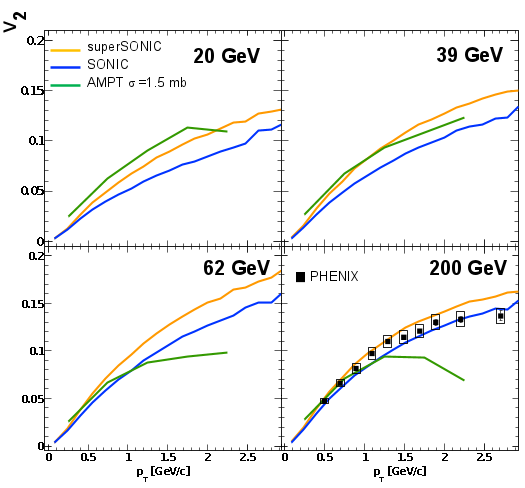
\includegraphics[width=0.75\linewidth]{figs/dau_bescan_theory.png}
\caption{Calculations of $v_2(\pt)$ \dau events at various \sqsn (given on the upper right of each panel) for AMPT, SONIC, and SuperSONIC models. Note that there are data points in the lower right panel due to the fact that the $v_2$ in \dau at \sqsn = 200 GeV has been measured previously by PHENIX from data taken in 2008~\cite{PhysRevC.93.044910}.}
\label{fig:dau_bes_predictions}
\end{center}
\end{figure}
